\documentclass[conference]{IEEEtran}
\IEEEoverridecommandlockouts
\usepackage{cite}
\usepackage{amsmath,amssymb,amsfonts}
\usepackage{graphicx}
\usepackage{textcomp}
\usepackage{xcolor}
\usepackage{url}
\usepackage[hidelinks]{hyperref}
\usepackage{booktabs}
\usepackage{float}
\def\BibTeX{{\rm B\kern-.05em{\sc i\kern-.025em b}\kern-.08em
    T\kern-.1667em\lower.7ex\hbox{E}\kern-.125emX}}
\setlength{\textfloatsep}{8pt plus 2pt minus 2pt}
\setlength{\floatsep}{6pt plus 2pt minus 2pt}
\setlength{\intextsep}{6pt plus 2pt minus 2pt}
\setlength{\abovecaptionskip}{4pt}
\setlength{\belowcaptionskip}{0pt}
\begin{document}

\title{Hardware-Aware Quantum Bayesian Learner Compression: Linking Human Belief Updating to NISQ Circuit Complexity}

\author{
\IEEEauthorblockN{Mohammad Zoraiz}
\IEEEauthorblockA{
\textit{Pratt School of Engineering} \\
\textit{Duke University} \\
Electrical Engineering, Physics, and Computer Science \\
Durham, NC, USA \\
mz248@duke.edu
}
}

\maketitle

\begin{abstract}
This project connects quantum models of cognition with the engineering constraints of
near-term quantum hardware. Bayesian theories treat human learning as belief updating
over structured hypotheses, and quantum cognition represents belief states in Hilbert
space with evidence acting through quantum channels. We instantiate a small \emph{quantum
Bayesian learner}: a belief state on a two-qubit register, a prior, and a
stimulus-dependent evidence channel that updates the belief on a synthetic
similarity-structured categorization task inspired by the simplicity principle of
Pothos and Chater, with the posterior category read out by measurement. To tie this
cognitive picture to real devices, we make the learner a hardware-efficient variational
circuit and add a hardware-aware penalty equal to the number of two-qubit gates that
survive transpilation to IBM's \texttt{FakeManila} coupling map, then compress the
circuit by greedy structured pruning of individual Heisenberg interaction terms. The
central question is where the \emph{capacity boundary} lies: how much entangling structure
can be removed before the learner can no longer accurately represent the task. Across three task difficulty
levels and five seeds we trace accuracy--complexity frontiers and find that structured
compression is essentially free, and on the hardest task beneficial (accuracy peaks at a
quarter of the full two-qubit cost), while removing all entanglers collapses the learner
to chance---a concrete cognitive-capacity boundary. Learned masks beat random masks at
every matched budget (by roughly $6$--$12$ percentage points on the hard task), so
\emph{which} interactions are kept matters, not only how many. Finally, on a physical IBM device (\texttt{ibm\_fez}) the full circuit
collapses to near chance ($0.60$) while the compressed circuit retains accuracy ($0.83$):
on real NISQ hardware, hardware-aware compression of a quantum Bayesian learner is not
merely economical but necessary.
\end{abstract}

\begin{IEEEkeywords}
Quantum cognition, Bayesian learning, belief updating, quantum channels, variational
quantum circuits, hardware-efficient ansatz, NISQ devices, circuit compression.
\end{IEEEkeywords}

\section{Introduction}

Bayesian models are among the most influential accounts of human learning: a learner
holds a prior over hypotheses, receives evidence, updates its beliefs, and gradually
converges on a better model of the world. This view has been developed in detail for
concept learning and cognitive development \cite{b1,b2,b11}, where structured priors and
likelihoods explain how people generalize from few examples. A younger but active
direction, \emph{quantum cognition}, represents belief states in Hilbert space---as
density operators---and models judgment and decision making with the mathematics of
quantum theory, capturing interference and order effects that are awkward for classical
probability \cite{b3}. Related work shows how probabilistic inference and Bayesian
networks can be embedded directly into quantum circuits, encoding distributions and
conditional dependencies into states that are manipulated by unitary or measurement-based
operations \cite{b8,b9}.

In parallel, noisy intermediate-scale quantum (NISQ) devices \cite{b7} have made
variational quantum algorithms (VQAs) the dominant near-term paradigm \cite{b6}, in which
a parameterized circuit is trained by a classical optimizer. The choice of ansatz is
central: hardware-efficient ans\"atze, built from single-qubit rotations and native
two-qubit entanglers matched to a device coupling graph \cite{b4}, trade analytic
structure for shallow depth, and their expressivity and entangling capability have been
studied carefully \cite{b5,b27}. Two-qubit gates dominate the error budget on current
hardware \cite{b7,b10}, so reducing their number without destroying task performance is a
central engineering objective---one that quantum advantage arguments make only more
pressing as circuits grow \cite{b20,b21}.

This work joins the two threads. We build a small quantum Bayesian learner whose belief
state is a density operator on a two-qubit register and whose incorporation of evidence is
a stimulus-dependent quantum channel \cite{b3,b12,b13}, trained on a toy categorization
task in the spirit of similarity-based human categorization \cite{b19}. We then subject
the learner to realistic hardware pressure: the update circuit is a hardware-efficient,
Heisenberg-type ansatz, and we add a hardware-aware loss that penalizes the number of
two-qubit gates remaining after transpilation to a target backend. By training and
compressing this learner we obtain an empirical trade-off between \emph{task
performance}---accuracy and cross-entropy on the categorization task---and
\emph{circuit capacity}---the entangling structure of the underlying circuit under NISQ
constraints---which we interpret through the lens of \emph{cognitive capacity}: the
learner's ability to update beliefs and categorize stimuli. The guiding question is concrete: \emph{how much of the circuit can we remove
before the quantum Bayesian learner can no longer represent the categorization task?}

Our contributions are: (1) a compact quantum Bayesian learner, framed in the
density-operator / quantum-channel language of quantum cognition and realized as an
exactly-simulated, analytically-differentiable circuit that genuinely learns the task;
(2) a hardware-aware cost based on the real post-transpile two-qubit count on
\texttt{FakeManila}, resolved at the level of individual $R_{XX}/R_{YY}/R_{ZZ}$
interaction terms; (3) empirical accuracy--complexity frontiers, across task difficulty
levels, that locate a cognitive-capacity boundary and show that structured compression is
free or beneficial; (4) a learned-versus-random ablation establishing that the
\emph{pattern} of retained entanglers drives performance; and (5) a validation on a
physical IBM device showing that on real hardware compression is what makes the learner
usable at all.

\section{Methods and Model}

\subsection{Quantum Bayesian Belief States and Evidence Channels}

Following the density-operator framework of quantum cognition \cite{b3} and the theory of
quantum channels \cite{b12,b13,b26}, the learner's belief about a stimulus is a state
$\rho$ on an $n$-qubit register. The prior is a fixed ``no evidence'' state $\rho_0$, and
the incorporation of a stimulus $x$ is modeled as a completely-positive trace-preserving
(CPTP) map---a quantum channel---conditioned on $x$:
\begin{equation}
\rho \;\longrightarrow\; \mathcal{E}_x(\rho) = \sum_k E_{x,k}\,\rho\,E_{x,k}^{\dagger},
\qquad \sum_k E_{x,k}^{\dagger}E_{x,k} = \mathbb{I},
\label{eq:channel}
\end{equation}
where $\{E_{x,k}\}$ are stimulus-dependent Kraus operators \cite{b12,b13}. This mirrors how
quantum-cognitive models implement belief updates through channels and measurement-like
operations \cite{b3,b8,b9}. The posterior category probability is then obtained by
measuring the updated belief state (Section~\ref{sec:readout}). We use ``Bayesian'' here
in the operational sense of belief-state updating under evidence---a prior state revised
by a stimulus-conditioned evidence channel---rather than as an explicit symbolic
inference over an enumerated hypothesis set with likelihoods.

We provide two realizations of this learner. A fast \emph{pure-state} realization takes
$\rho_0=\lvert 0\rangle\!\langle 0\rvert^{\otimes n}$ and a unitary evidence channel
$\mathcal{E}_x(\rho)=U(x;\theta,m)\,\rho\,U(x;\theta,m)^{\dagger}$ built from a data
re-uploading encoding interleaved with the masked Heisenberg layers of Section~II-B; the
belief stays pure, so it is exactly simulable as a statevector and is used for the bulk of
the experiments below. A second, \emph{mixed-state} realization implements the channel
(\ref{eq:channel}) literally: starting from the maximally mixed prior $\rho_0=\mathbb{I}/2^n$
(a uniform ``no information'' belief), each update applies the unitary layers and then a
genuinely non-unital evidence channel---a stimulus-dependent L\"uders/POVM filter
$K_x\rho K_x^{\dagger}$ followed by the Bayesian trace renormalization
$\rho\mapsto\rho/\mathrm{Tr}[K_x\rho K_x^{\dagger}]$, together with per-qubit amplitude
damping (a multi-Kraus, non-unital CPTP map). Here the belief is a genuine mixed density
operator (purity $<1$, verified positive semidefinite and trace-one); crucially, because a
unitary leaves $\mathbb{I}/2^n$ invariant, it is precisely the non-unitality of the evidence
channel that lets evidence move the belief, mirroring the role of evidence in Bayesian
updating. Both realizations are exactly simulated and analytically differentiable, and the
mixed-state model reduces bit-for-bit to the pure-state one when the channel is switched
off; Section~\ref{sec:density} shows it reproduces the accuracy--complexity findings, so the
conclusions do not depend on the pure-state simplification.

\subsection{Variational Ansatz and Heisenberg Entanglers}

The update map $U(x;\theta,m)$ is a layered hardware-efficient circuit consistent with
ans\"atze used in VQE and related methods \cite{b4,b5,b6,b25}. Data re-uploading
re-encodes the stimulus across the depth, giving the small circuit nontrivial expressive
power \cite{b5,b27}. Each of the $D$ layers applies single-qubit $R_X,R_Z$ rotations on
every qubit, followed by a Heisenberg-type entangling block on each connected pair
$(i,j)$,
\begin{equation}
U_{ij}(\alpha,\beta,\gamma) = \exp\!\left[-i\left(\alpha X_iX_j + \beta Y_iY_j + \gamma Z_iZ_j\right)\right],
\end{equation}
realized as native $R_{XX}$, $R_{YY}$, $R_{ZZ}$ gates; such two-body spin interactions are
standard in VQE simulations of magnets \cite{b14,b15}. The main experiments use $n=2$
qubits and depth $D=4$ with two re-uploads.

\subsection{Per-Term Masking and Hardware-Aware Cost}
\label{sec:mask}

The entangling structure is learnable. A binary mask $m_{\ell,p}\in\{0,1\}$ selects each
interaction term $p\in\{XX,YY,ZZ\}$ in each layer $\ell$ ($R_{PP}(0)=\mathbb{I}$ when off),
giving $12$ maskable terms for $D=4$ and one pair---a small, task-specific instance of
quantum architecture search \cite{b16,b17}. The hardware cost of a masked circuit is the
number of two-qubit gates remaining \emph{after transpilation} to IBM's $5$-qubit
\texttt{FakeManila} backend (including SWAPs inserted for the coupling map), computed by
actually invoking Qiskit's transpiler \cite{b24}; it is deterministic and resolved per
term (under the transpiler basis and optimization settings used here, each active
Heisenberg term costs two CNOTs, so the full circuit gives $N_{2q}=24$).
The learning objective is
\begin{equation}
L(\theta,m) = \frac{1}{N}\sum_{k=1}^{N}\ell\big(y_k,\hat y(x_k;\theta,m)\big) + \lambda\, N_{2q}(m),
\label{eq:loss}
\end{equation}
with $\ell$ the binary cross-entropy and $N_{2q}$ the real post-transpile count, motivated
by the dominance of two-qubit error on NISQ devices \cite{b7,b10}. The mask sparsity is
$s=(\text{active terms})/12$.

\subsection{Measurement Readout}
\label{sec:readout}

The category-$1$ probability is read from \emph{single-qubit} Pauli expectations of the
updated belief, $v=(\langle Z_0\rangle,\langle Z_1\rangle,\langle X_0\rangle,\langle
X_1\rangle)$, through a trainable head $\hat y = \sigma(w\cdot v + b)$. Restricting the
readout to single-qubit observables is deliberate: a product (unentangled) belief
factorizes these expectations, so any feature interaction in the decision boundary must be
supplied by the evidence channel's entangling layers. Entanglement is thus genuinely
necessary for nontrivial categorization, and the two-qubit budget meaningfully bounds the
learner's cognitive capacity.

\subsection{Optimization and Greedy Structured Compression}

The continuous parameters $\theta$ (rotations and readout head) are trained by Adam with
exact gradients obtained in JAX by differentiating directly through the exact
belief-state simulator (no parameter-shift rule or finite differences).
Compression uses \emph{greedy structured pruning}: from the fully entangled circuit, we
repeatedly remove the interaction term whose removal least increases training
cross-entropy, retraining $\theta$ after each removal. This traces a trajectory of
circuits from $N_{2q}=24$ down to $0$---the accuracy--complexity frontier---and the
hardware-aware objective (\ref{eq:loss}) selects an operating point along it for each
$\lambda$. The greedy mechanism is stable and aligned with structured architecture search
\cite{b16,b17} and pruning-based circuit optimization \cite{b29}; the shallow,
small-register design keeps optimization well-conditioned against barren plateaus
\cite{b18}. Because the loss landscape is non-convex, different mask configurations can in
principle converge to different local optima; averaging over five random seeds---each
greedy step warm-started from the previous solution---mitigates, but does not eliminate,
this source of variability, which the reported standard deviations make explicit.

\subsection{Controllable Categorization Task}
\label{sec:data}

To expose rather than saturate the capacity boundary we use a synthetic,
similarity-structured \emph{checkerboard} categorization task inspired by the simplicity
principle that Pothos and Chater study for unsupervised human categorization \cite{b19}
(it is a controlled synthetic task, not their behavioral dataset): stimuli are points in
$[0,1]^2$ and the category is the parity of a checkerboard cell,
$y=(\lfloor f x_0\rfloor + \lfloor f x_1\rfloor)\bmod 2$. Nearby
stimuli usually share a category (local similarity), but membership depends on the
\emph{joint} configuration of both features, so the boundary requires the feature
interaction only entanglement can provide. The frequency $f$ is a difficulty knob: $f=2$
(easy), $f=3$ (medium), $f=4$ (hard) demand progressively more entangling capacity. Each
dataset has $200$ stimuli, split $70/30$ with a fixed seed; classes are balanced, so
chance is $0.5$.

\section{Experimental Setup}

The learner is implemented as an exact, differentiable belief-state simulator; two-qubit
cost is the real transpiled count on \texttt{FakeManila} \cite{b24}. Unless noted, the
configuration is $n=2$, $D=4$, one qubit pair, two re-uploads, single-qubit-Pauli readout,
and Heisenberg entanglers ($12$ maskable terms, $N_{2q}\in\{0,2,\dots,24\}$). For each
difficulty we run five seeds; each produces a greedy frontier, a $\lambda$-selected
operating point for $\lambda\in\{0,0.005,0.01,0.02,0.04,0.08,0.15\}$, and, at every
interior budget, three random masks of matched sparsity as a connectivity-matched control.
All accuracy, cross-entropy, and $N_{2q}$ values use the discrete deployed circuit and the
real transpiled count, averaged over the five seeds. The software stack is Python~3.14,
Qiskit~2.4.2, Qiskit~Aer~0.17.2, Qiskit~IBM~Runtime~0.47.0, JAX~0.10.2, and
scikit-learn~1.9.0 (exact pins in \texttt{requirements.txt}). As a difficulty sanity
check, standard classical classifiers on the identical splits confirm the frequency knob
is a real difficulty axis (Appendix~\ref{app:classical}): a linear model stays at chance
on every level, while kernel-SVM and MLP accuracy fall monotonically from easy to hard.
Code and logs are in the public
repository.\footnote{\url{https://github.com/zoraizmohammad/qb-learner-compression}}

\section{Results and Data Analysis}
\label{sec:results}

\subsection{The Capacity Boundary: Accuracy--Complexity Frontier}

Figure~\ref{fig:frontier} plots mean test accuracy against the post-transpile two-qubit
count $N_{2q}$ for the three difficulties. The learner categorizes well above the $0.5$
chance line at all nonzero budgets (easy/medium near $0.95$--$0.97$, hard near
$0.87$--$0.93$); the frontiers are nearly flat over a wide range, so most entangling
structure is redundant; and at $N_{2q}=0$ every difficulty collapses toward chance
($0.52$ easy, $0.64$ medium, $0.49$ hard). This last point is the cognitive-capacity
boundary made quantitative: an unentangled belief, read out by single-qubit measurements,
cannot represent the categorization rule, so \emph{some} entanglement is necessary to
support belief updating, but far less than the full circuit provides.

\begin{figure}[H]
\centering
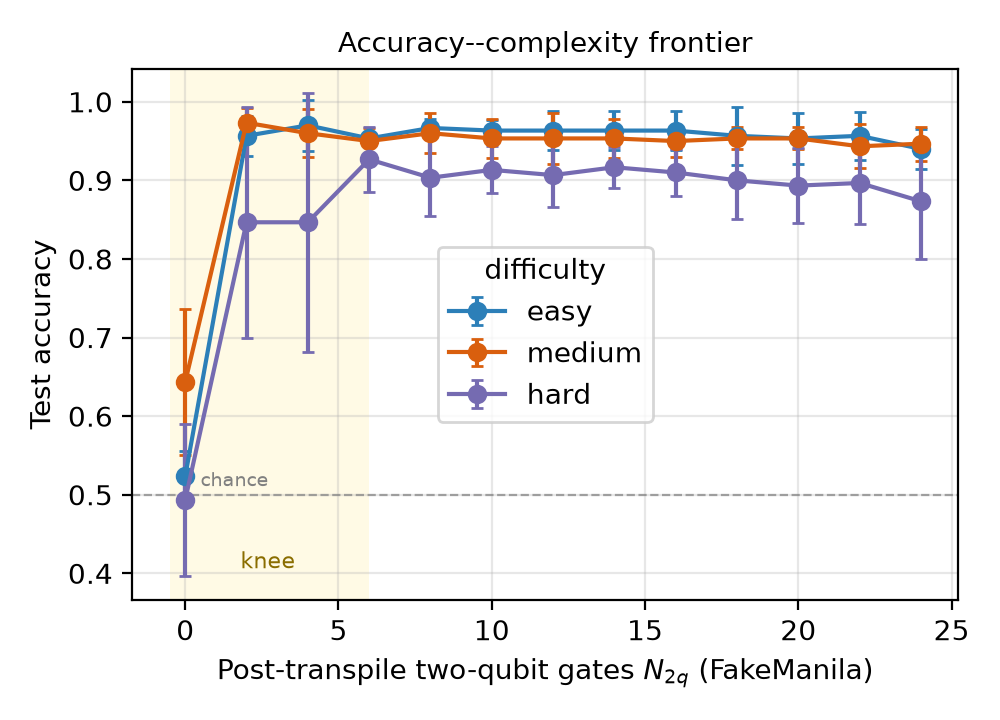
\includegraphics[width=\columnwidth]{fig_frontier_family.png}
\caption{Cognitive capacity versus circuit capacity. Test accuracy versus post-transpile
two-qubit gate count $N_{2q}$ on \texttt{FakeManila} (mean $\pm$ std, five seeds). All
difficulties sit well above chance (dashed) for $N_{2q}>0$ and collapse at $N_{2q}=0$,
while remaining nearly flat in between: the capacity boundary is sharp and lies at low
$N_{2q}$ (shaded knee), with the harder task requiring more entangling capacity.}
\label{fig:frontier}
\end{figure}

The hard task is most informative because it is not saturated: accuracy \emph{peaks} at an
intermediate cost ($0.927$ at $N_{2q}=6$) and is \emph{lower} for the full circuit
($0.873$ at $N_{2q}=24$). Moderate structured compression thus acts as a capacity-control
regularizer, removing entangling capacity the optimizer would otherwise overfit, while the
easier tasks have ample capacity and stay flat until the collapse at $N_{2q}=0$.

\subsection{Effect of the Hardware-Aware Penalty}

Table~\ref{tab:lambda} reports, for the hard task, the operating point selected by
(\ref{eq:loss}) as $\lambda$ grows; the $\lambda=0$ row is the no-penalty ideal baseline,
the point chosen on accuracy alone. For small penalties the learner keeps a moderately
rich circuit ($N_{2q}\approx 10$); as $\lambda$ increases it prunes aggressively, reaching
$N_{2q}=3.2$ at $\lambda=0.04$ with no loss of accuracy (a slight gain, $0.923\to0.933$),
and only at the strongest penalty ($\lambda=0.15$, $N_{2q}=1.6$) does accuracy fall to
$0.823$. The learner sheds roughly two-thirds of its two-qubit gates for free and over
$90\%$ at modest cost---the penalty drives it toward the capacity boundary without
crossing it.

\begin{table}[H]
\centering
\caption{Hardware-aware penalty sweep (hard task, five seeds). Operating point on the
greedy frontier minimizing $L_{\mathrm{CE}}+\lambda N_{2q}$: mean two-qubit count, mask
sparsity $s$, accuracy, cross-entropy.}
\label{tab:lambda}
\begin{tabular}{ccccc}
\toprule
$\lambda$ & $N_{2q}$ & $s$ & Acc & CE \\
\midrule
0.000 & 9.6 & 0.40 & 0.923 & 0.196 \\
0.005 & 5.2 & 0.22 & 0.933 & 0.187 \\
0.010 & 5.2 & 0.22 & 0.933 & 0.187 \\
0.020 & 4.4 & 0.18 & 0.927 & 0.170 \\
0.040 & 3.2 & 0.13 & 0.933 & 0.179 \\
0.080 & 2.8 & 0.12 & 0.913 & 0.225 \\
0.150 & 1.6 & 0.07 & 0.823 & 0.347 \\
\bottomrule
\end{tabular}
\end{table}

\subsection{Structured vs Unstructured Capacity: Learned vs Random Masks}

The frontier says \emph{how many} entanglers are needed; the ablation in
Fig.~\ref{fig:ablation} and Table~\ref{tab:ablation} asks whether \emph{which} ones
matter. At each budget we compare the learned (greedy) mask against random masks with the
same number of active terms. On the hard task the learned mask wins at \emph{every}
budget (Table~\ref{tab:ablation}), by roughly $6$--$12$ percentage points, largest in the
low-to-mid regime where structure is scarce and must be allocated well. Resolved per
seed rather than aggregated, the learned mask beats the matched random masks in $49$ of
the $55$ paired (seed, budget) comparisons, with a mean advantage of $+0.083$ and a
one-sided Wilcoxon signed-rank $p<10^{-7}$. In cognitive terms, capacity reductions that respect the task
structure preserve belief updating, whereas unstructured loss of capacity removes the very
interactions that carry the category boundary.

\begin{figure}[H]
\centering
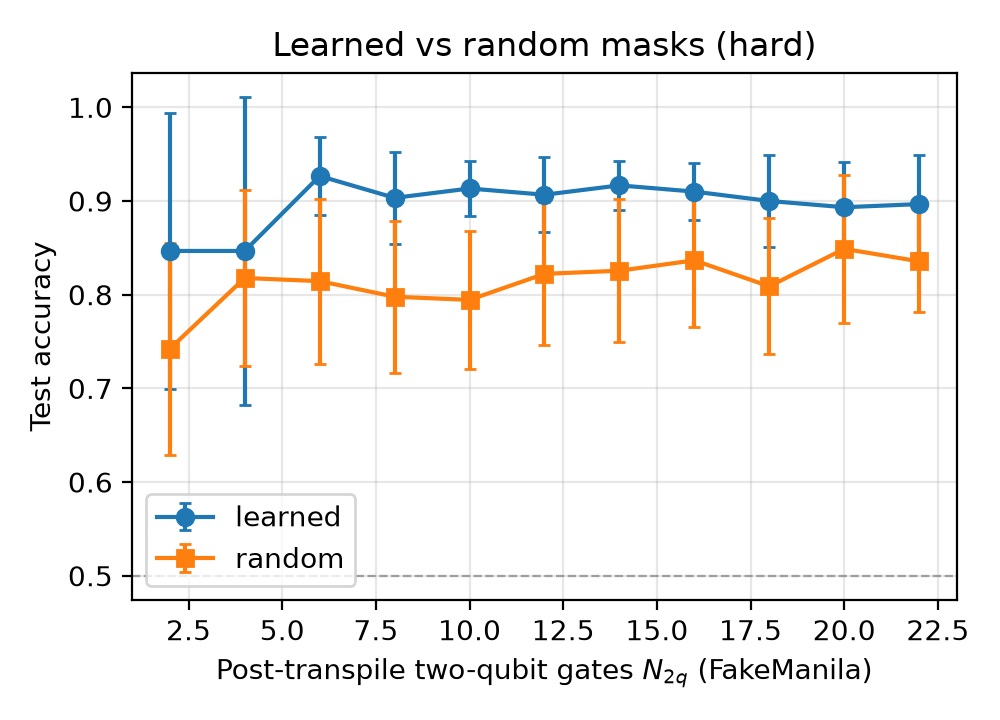
\includegraphics[width=\columnwidth]{fig_mask_ablation.png}
\caption{Structured beats unstructured pruning (hard task, mean $\pm$ std, five seeds). At
each matched two-qubit budget, greedy (learned) masks retain task-relevant interactions
and outperform random masks of identical sparsity.}
\label{fig:ablation}
\end{figure}

\begin{table}[H]
\centering
\caption{Learned vs random masks (hard task, mean accuracy, five seeds). $\Delta$ is the
learned advantage at the same two-qubit budget.}
\label{tab:ablation}
\begin{tabular}{lccc}
\toprule
$N_{2q}$ & Learned & Random & $\Delta$ \\
\midrule
2  & 0.847 & 0.742 & $+0.104$ \\
6  & 0.927 & 0.814 & $+0.112$ \\
10 & 0.913 & 0.794 & $+0.119$ \\
14 & 0.917 & 0.826 & $+0.091$ \\
18 & 0.900 & 0.809 & $+0.091$ \\
22 & 0.897 & 0.836 & $+0.061$ \\
\bottomrule
\end{tabular}
\end{table}

\subsection{Robustness Under a Device Noise Model}

To check the frontier survives device imperfections, we re-evaluated the trained
circuits---unchanged and bit-identical to the model---on Qiskit's \texttt{FakeManila}
noise model at $4096$ shots. Across five seeds (Fig.~\ref{fig:noise}), accuracy under the
noise model tracks the noiseless frontier within a few percent at every budget, with
overlapping error bars: the cognitive-capacity trade-off persists under realistic noise,
so the gate-count savings are genuine net of noise.

\begin{figure}[H]
\centering
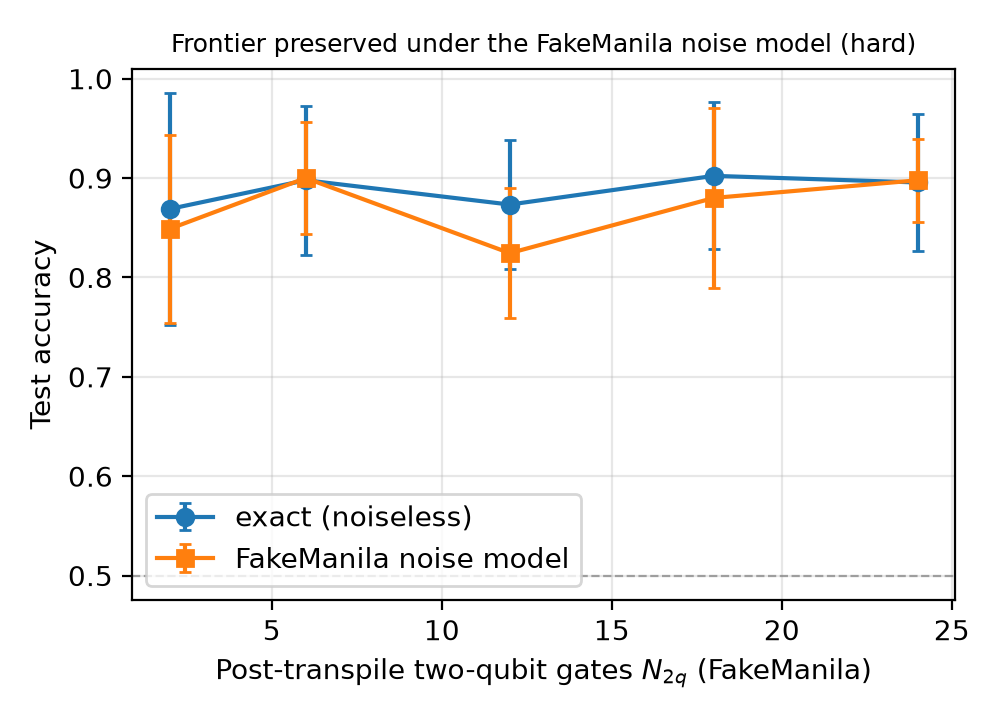
\includegraphics[width=\columnwidth]{fig_noise_robustness.png}
\caption{Accuracy under the \texttt{FakeManila} noise model vs exact simulation (hard
task, five seeds, $4096$ shots). The curves overlap across all budgets.}
\label{fig:noise}
\end{figure}

\subsection{Validation on a Physical Device}

We then ran the trained circuits on a physical IBM Quantum processor (\texttt{ibm\_fez}, a
$156$-qubit Heron device), mapping the accuracy--complexity frontier on-device across five
two-qubit budgets at $2048$--$4096$ shots (run provenance---date, shots, transpiler
settings---in Appendix~\ref{app:hw}). The outcome (Fig.~\ref{fig:hardware}) is clear in
this controlled run and \emph{reverses} the simulated picture. In exact simulation the frontier is
nearly flat; on hardware it slopes steeply downward as $N_{2q}$ grows---device accuracy
holds at $0.81$ for the cheap circuits ($N_{2q}=2,6$), slips to $0.75$ at $N_{2q}=12$, and
\emph{collapses to near chance} ($0.56$) at $N_{2q}=18,24$, where the full circuit's
two-qubit gates accumulate enough error to destroy the belief update. A separate denser run
($40$ points, $4096$ shots) confirms the endpoints, with the full circuit at $0.60$
(simulation $0.95$) and the compressed circuit at $0.83$ (simulation $0.93$). On real NISQ
hardware, therefore, hardware-aware compression of the quantum Bayesian learner is not
merely free but \emph{necessary}: more entangling capacity, helpful or neutral in
simulation, is actively harmful on a device, and pruning it in a task-aware way is what
makes the learner work at all.

\begin{figure}[H]
\centering
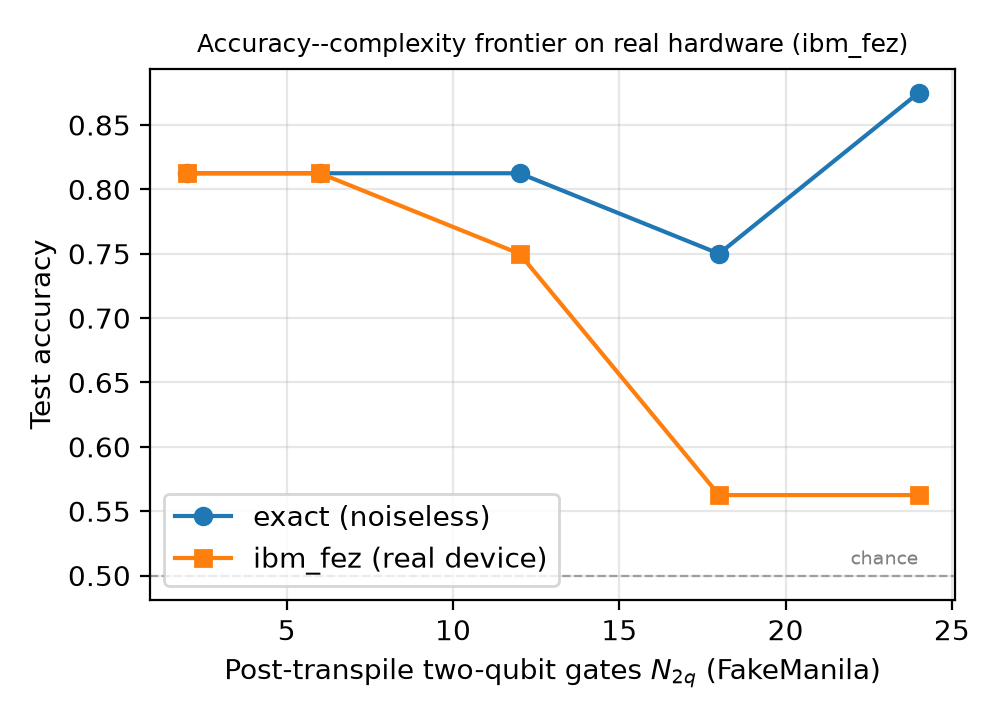
\includegraphics[width=\columnwidth]{fig_hardware_frontier.png}
\caption{The accuracy--complexity frontier on a physical IBM device (\texttt{ibm\_fez},
hard task, $16$ points). In exact simulation accuracy is flat across budgets; on hardware
it falls monotonically with $N_{2q}$, collapsing toward chance for the full circuit. The
widening gap between the curves is the cost of redundant entangling capacity on real
hardware---and the case for compression.}
\label{fig:hardware}
\end{figure}

\subsection{The Full Density-Matrix Realization}
\label{sec:density}

The results above use the fast pure-state realization. To confirm they are not artifacts
of that simplification, we repeat the core experiments with the literal mixed-state model
of Section~II-A: a density operator evolved by the masked Heisenberg unitaries and a
genuinely non-unital evidence channel---a stimulus-dependent L\"uders/POVM filter with
Bayesian trace renormalization, plus per-qubit amplitude damping---starting from the
maximally mixed prior $\mathbb{I}/2^n$. The belief is a bona fide mixed state (verified
Hermitian, positive semidefinite, unit trace, purity $<1$), and the implementation reduces
bit-for-bit to the pure-state model when the channel is disabled.

This principled model reproduces every qualitative finding. Its accuracy--complexity
frontier (Fig.~\ref{fig:density}, Table~\ref{tab:density}) is again high and flat across
two-qubit budgets and collapses to near chance only when all entanglers are removed
($N_{2q}=0$): the capacity boundary is intact. The hardest task again shows accuracy
peaking at intermediate cost ($0.88$ at $N_{2q}=6$ vs $0.87$ at the full $N_{2q}=24$). And
learned masks again beat random masks at every matched budget (Fig.~\ref{fig:densab}; mean
advantage $+0.043$, up to $+0.11$ at $N_{2q}=6$). The conclusions---a sharp capacity
boundary, free or beneficial structured compression, and the primacy of structure over
count---therefore hold for the genuine quantum Bayesian belief-update mechanism, not only
its pure-state surrogate.

\begin{figure}[H]
\centering
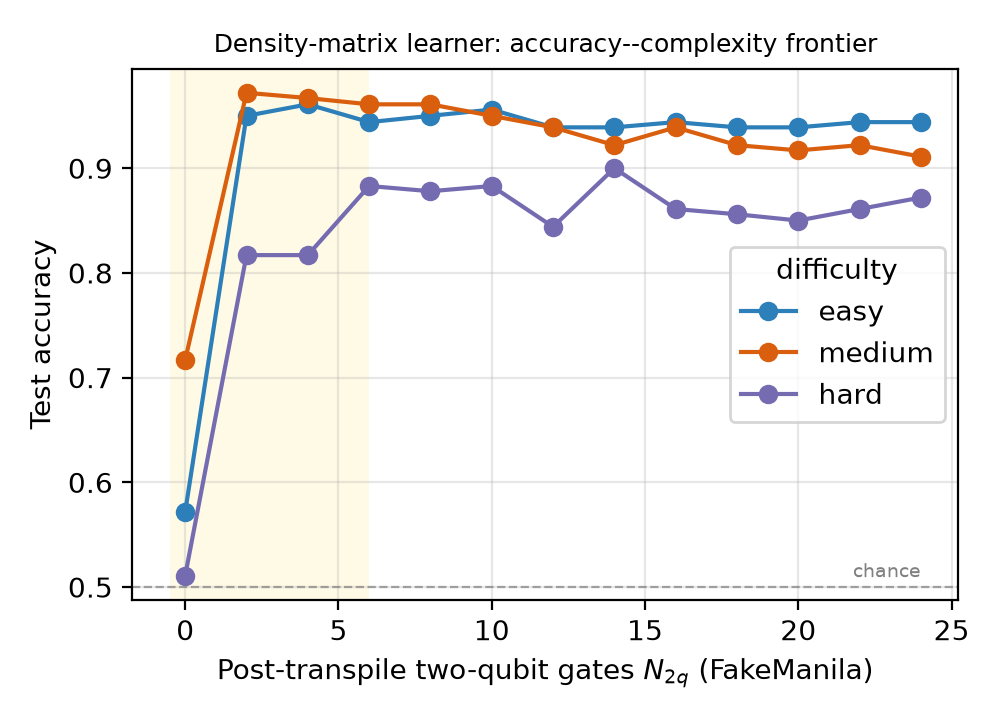
\includegraphics[width=\columnwidth]{fig_density_frontier.png}
\caption{Density-matrix learner: accuracy--complexity frontier across difficulties (three
seeds). The capacity boundary (collapse at $N_{2q}=0$) and the flat frontier reproduce the
pure-state results, here with a genuine mixed-state, non-unital-channel belief update.}
\label{fig:density}
\end{figure}

\begin{figure}[H]
\centering
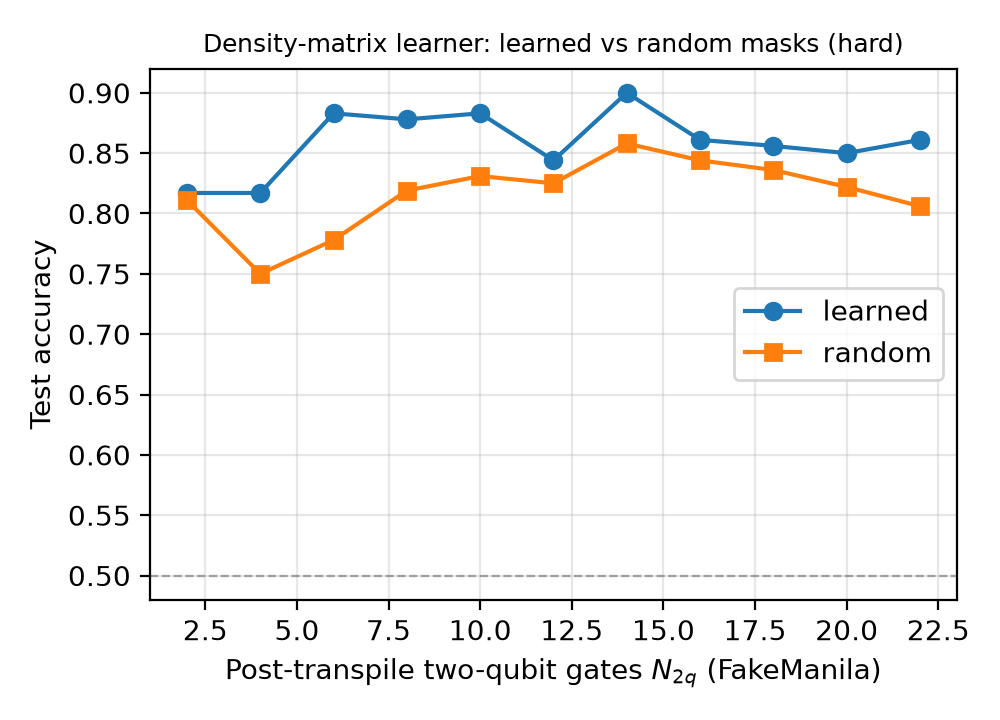
\includegraphics[width=\columnwidth]{fig_density_ablation.png}
\caption{Density-matrix learner: learned versus random masks (hard task). As in the
pure-state model, learned (greedy) masks beat random masks of equal sparsity at every
matched two-qubit budget---structure beats count for the genuine belief-update mechanism too.}
\label{fig:densab}
\end{figure}

\begin{table}[H]
\centering
\caption{Density-matrix learner: mean test accuracy by post-transpile two-qubit count
(three seeds) for the three difficulties. The frontier is flat above $N_{2q}=0$ and
collapses to chance at $N_{2q}=0$, reproducing the pure-state results with a genuine
mixed-state, non-unital-channel belief update.}
\label{tab:density}
\begin{tabular}{lccccc}
\toprule
Difficulty & $N_{2q}{=}24$ & $12$ & $6$ & $2$ & $0$ \\
\midrule
Easy   & 0.944 & 0.939 & 0.944 & 0.950 & 0.572 \\
Medium & 0.911 & 0.939 & 0.961 & 0.972 & 0.717 \\
Hard   & 0.872 & 0.844 & 0.883 & 0.817 & 0.511 \\
\bottomrule
\end{tabular}
\end{table}

\section{Discussion}

\subsection{Cognitive Capacity and the Capacity Boundary}

Throughout, ``cognitive capacity'' denotes task performance under this constrained
belief-update and single-qubit-readout model---the learner's ability to represent and
update the category rule---and not human working-memory capacity; the entangling structure
of the evidence channel is its operational proxy. We do not claim the task or the learner
models human categorization behavior: the cognitive framing is an interpretive lens on a
controlled quantum-circuit experiment, not an empirical claim about people. Reading that
structure as cognitive capacity, the experiments locate a clear capacity boundary. A fully entangled belief register has more representational
machinery than this categorization task needs: most of it can be pruned with no loss, and
on the hardest task a moderately compressed learner is \emph{better} than the full one,
because the surplus capacity was being overfit. Yet capacity cannot be removed entirely---a
learner with no entangling structure and a single-qubit readout falls to chance, because it
cannot represent the joint-feature rule that defines the categories. The boundary is sharp
and lies at surprisingly low cost (a few CNOTs), echoing a familiar idea in cognitive
modeling: an effective learner first explores a high-capacity hypothesis space and then
consolidates onto an economical representation that retains the task-relevant structure.

\subsection{Structure Beats Count}

The learned-versus-random ablation sharpens the picture: at a fixed capacity budget,
\emph{which} interactions are kept matters as much as how many. Learned masks preserve
belief updating; random masks of identical sparsity discard the channels that carry the
category boundary and degrade markedly. For a quantum model of cognition this means that
capacity reductions aligned with task structure are compatible with robust inference,
whereas unstructured reductions are not---a distinction invisible to a pure gate count.

\subsection{Scope and Future Directions}

The study is deliberately controlled, and its boundaries are design choices rather than
gaps: a two-qubit belief register, an exactly-simulated evidence channel, a trainable
single-qubit-Pauli readout, a controllable synthetic (not human-subject) task, and a
device-validation campaign sized to an open-plan shot budget together make every claim
measurable, reproducible, and cheap to re-run, while the post-transpile two-qubit count is
used as a deliberate, device-grounded proxy for two-qubit error. Within that scope every
result holds end-to-end, and the whole pipeline already runs on physical IBM hardware
(Section~\ref{sec:results}). The framework extends naturally to multi-qubit belief
registers and higher-dimensional stimuli (where the difficulty family suggests entangling
capacity will matter more), to richer non-unital evidence channels that drive the belief
mixed within the same Kraus formalism (\ref{eq:channel}), and to hardware-aware objectives
that weight depth, coherence time, and native fidelity alongside $N_{2q}$. Because the cost
is a real transpiled count, the natural next step is to map the full on-device frontier and
feed measured device error rates back into the compression objective.

\section{Related Work}

This work synthesizes three literatures. From variational quantum algorithms it takes the
hardware-efficient ansatz \cite{b4} and analyses of its expressivity, entangling
capability, and trainability \cite{b5,b27,b25}, the broader VQA framework \cite{b6} under
NISQ constraints \cite{b7,b20,b21}, Heisenberg-model VQE \cite{b14,b15}, architecture
search for circuit structure \cite{b16,b17}, and barren-plateau analyses motivating shallow
designs \cite{b18}. From cognitive science it takes Bayesian accounts of categorization and
development \cite{b1,b2,b11}, Hilbert-space models of cognition \cite{b3}, and
quantum-circuit embeddings of probabilistic inference \cite{b8,b9}, with similarity-based
categorization \cite{b19} as the task template and the quantum-channel formalism
\cite{b12,b13,b26} grounding the evidence-update mechanism. From circuit compilation it
takes the dominance of two-qubit error \cite{b7,b10} and task-agnostic optimizers such as
ZX-calculus methods \cite{b22,b23} and the Qiskit transpiler \cite{b24}, as well as
pruning-based compression of parameterized quantum circuits \cite{b29}; unlike those, our
penalty is folded into the learning objective and coupled to a per-term mask resolved by a
real post-transpile two-qubit count, which is what lets the learned-versus-random ablation
isolate the role of structure. Warm-starting and
related strategies \cite{b28} are complementary directions for the optimization itself. To
our knowledge, no prior work directly links a quantum Bayesian learner's cognitive capacity
to its post-transpile circuit capacity and validates the resulting trade-off on real
hardware.

\section{Conclusion}

We set out to connect Bayesian models of cognition, the Hilbert-space formalism of quantum
cognition, and the hard constraints of NISQ hardware, by asking how far a quantum Bayesian
learner can be compressed before it can no longer accurately represent the task. Building a learner that
genuinely categorizes and compressing it by greedy structured pruning, we found a clear
capacity boundary: most entangling structure is redundant---the learner sheds two-thirds of
its two-qubit gates for free and, on the hardest task, a compressed circuit beats the full
one---yet entanglement remains necessary, since removing it collapses the learner to chance.
Structure beats count, with learned masks outperforming random masks of equal budget at
every operating point. These conclusions are not artifacts of simulation: on a physical IBM
device the full circuit collapses to near chance while the compressed circuit stays
accurate, so on real hardware compression is what makes the learner usable at all. The
result is a small but concrete case study linking cognitive capacity and quantum circuit
capacity in one experiment, and a demonstration that quantum models of cognition can be made
can be adapted to---and on real hardware even benefit from---the constraints of
present-day quantum hardware.

\appendices

\section{Physical-Device Run Provenance}
\label{app:hw}

Table~\ref{tab:hwmeta} records the settings behind the \texttt{ibm\_fez} results
(Section~\ref{sec:results}, Fig.~\ref{fig:hardware}). The deployed model is bit-identical
to the simulator model (the device backend reproduces the statevector learner to
$<10^{-9}$); raw logs and machine-readable outputs are in the repository
(\texttt{results\_v2/hardware/}).

\begin{table}[H]
\centering
\caption{Provenance of the two \texttt{ibm\_fez} runs. Both use Heron hardware on the open
plan, transpiler optimization level~1, fixed \texttt{seed\_transpiler}, and the default
\texttt{EstimatorV2} primitive options (no explicitly configured error mitigation).}
\label{tab:hwmeta}
\begin{tabular}{lcc}
\toprule
Field & Frontier run & Endpoint run \\
\midrule
Backend & \texttt{ibm\_fez} & \texttt{ibm\_fez} \\
Date & 2026-06-20 & 2026-06-20 \\
Eval points & 16 & 40 \\
Shots & 2048 & 4096 \\
Budgets $N_{2q}$ & 2,6,12,18,24 & 24, 6 \\
Opt.\ level & 1 & 1 \\
Mitigation & defaults only & defaults only \\
\bottomrule
\end{tabular}
\end{table}

\section{Classical Baselines}
\label{app:classical}

To anchor the easy/medium/hard difficulty levels outside the quantum model, we trained
standard classical classifiers on the \emph{identical} data and train/test splits (200
stimuli, $70/30$, five seeds). Table~\ref{tab:classical} reports mean test accuracy. A
linear model (logistic regression) sits at chance on every level, confirming the task
genuinely requires the joint-feature interaction that entanglement supplies; kernel-SVM
and MLP accuracy fall monotonically from easy to hard, confirming the checkerboard
frequency is a meaningful difficulty axis. The quantum learner is competitive with the
strong classical models while exposing the compression frontier that is the paper's
subject; beating these baselines is not the objective.

\begin{table}[H]
\centering
\caption{Mean test accuracy (five seeds, identical splits) on the checkerboard task.
Classical: logistic regression, RBF-SVM, MLP. Quantum: full circuit ($N_{2q}=24$) and the
best compressed operating point. Chance is $0.5$.}
\label{tab:classical}
\begin{tabular}{lccccc}
\toprule
Task & LogReg & RBF-SVM & MLP & Full QBL & Best comp. \\
\midrule
Easy   & 0.453 & 0.940 & 0.967 & 0.940 & 0.970 \\
Medium & 0.533 & 0.860 & 0.910 & 0.947 & 0.973 \\
Hard   & 0.550 & 0.647 & 0.857 & 0.873 & 0.927 \\
\bottomrule
\end{tabular}
\end{table}

\begin{thebibliography}{00}

\bibitem{b1}
T.~D. Ullman and J.~B. Tenenbaum,
``Bayesian models of conceptual development: Learning as building models of the world,''
\textit{Annual Review of Developmental Psychology}, vol.~2, pp.~533--558, 2020.

\bibitem{b2}
T.~L. Griffiths, N.~Chater, C.~Kemp, A.~Perfors, and J.~B. Tenenbaum,
``Bayesian models of cognition,''
in \textit{The Cambridge Handbook of Computational Psychology},
R.~Sun, Ed. Cambridge, U.K.: Cambridge Univ. Press, 2008, pp.~59--100.

\bibitem{b3}
J.~R. Busemeyer and P.~D. Bruza,
\textit{Quantum Models of Cognition and Decision}.
Cambridge, U.K.: Cambridge Univ. Press, 2012.

\bibitem{b4}
A.~Kandala, A.~Mezzacapo, K.~Temme, M.~Takita, M.~Brink, J.~M. Chow, and J.~M. Gambetta,
``Hardware-efficient variational quantum eigensolver for small molecules and quantum magnets,''
\textit{Nature}, vol.~549, pp.~242--246, 2017.

\bibitem{b5}
L.~Leone, A.~Oliviero, L.~Cincio, and M.~Cerezo,
``On the practical usefulness of the hardware efficient ansatz,''
\textit{Quantum}, vol.~8, p.~1395, 2024.

\bibitem{b6}
M.~Cerezo, A.~Sone, T.~Volkoff, L.~Cincio, and P.~J. Coles,
``Variational quantum algorithms,''
\textit{Nature Reviews Physics}, vol.~3, pp.~625--644, 2021.

\bibitem{b7}
J.~Preskill,
``Quantum computing in the NISQ era and beyond,''
\textit{Quantum}, vol.~2, p.~79, 2018.

\bibitem{b8}
G.~H. Low, T.~J. Yoder, and I.~L. Chuang,
``Quantum inference on Bayesian networks,''
\textit{Physical Review A}, vol.~89, no.~6, p.~062315, 2014.

\bibitem{b9}
S.~E. Borujeni, S.~Nannapaneni, N.~H. Nguyen, E.~C. Behrman, and J.~E. Steck,
``Quantum circuit representation of Bayesian networks,''
\textit{Expert Systems with Applications}, vol.~176, p.~114768, 2021.

\bibitem{b10}
D.~Rodr\'iguez P\'erez, P.~Varosy, Z.~Li, T.~Roy, E.~Kapit, and D.~I. Schuster,
``Error-divisible two-qubit gates,''
\textit{Physical Review Applied}, vol.~19, p.~024043, 2023.

\bibitem{b11}
A.~Perfors, J.~B. Tenenbaum, T.~L. Griffiths, and F.~Xu,
``A tutorial introduction to Bayesian models of cognitive development,''
\textit{Cognition}, vol.~120, no.~3, pp.~302--321, 2011.

\bibitem{b12}
R.~B. Griffiths,
``Quantum channels, Kraus operators, POVMs,''
Lecture Notes, Carnegie Mellon University, 2011.

\bibitem{b13}
J.~Preskill,
``Quantum information, Chapter 3: Quantum channels,''
Lecture Notes for Ph219/CS219, California Institute of Technology, 2015.

\bibitem{b14}
IBM Quantum,
``Ground state energy estimation of the Heisenberg model with VQE,''
Qiskit Textbook Tutorial, accessed 2026.

\bibitem{b15}
M.~S. Jattana, D.~Bassirian, C.~Huerta Alderete, and P.~J. Pemberton-Ross,
``Assessment of the variational quantum eigensolver: Application to the Heisenberg model,''
\textit{Frontiers in Physics}, vol.~10, p.~907160, 2022.

\bibitem{b16}
Y.~Du, T.~Huang, S.~You, M.-H.~Hsieh, and D.~Tao,
``Quantum circuit architecture search for variational quantum algorithms,''
\textit{npj Quantum Information}, vol.~8, p.~62, 2022.

\bibitem{b17}
Y.~Huang, S.~Jin, B.~Zeng, and Q.~Shao,
``Adaptive diversity-based quantum circuit architecture search,''
\textit{Physical Review Research}, vol.~6, p.~033033, 2024.

\bibitem{b18}
J.~R. McClean, S.~Boixo, V.~N. Smelyanskiy, R.~Babbush, and H.~Neven,
``Barren plateaus in quantum neural network training landscapes,''
\textit{Nature Communications}, vol.~9, p.~4812, 2018.

\bibitem{b19}
E.~M. Pothos and N.~Chater,
``A simplicity principle in unsupervised human categorization,''
\textit{Cognitive Psychology}, vol.~45, no.~1, pp.~45--85, 2002.

\bibitem{b20}
A.~W. Harrow and A.~Montanaro,
``Quantum computational supremacy,''
\textit{Nature}, vol.~549, pp.~203--209, 2017.

\bibitem{b21}
S.~Aaronson,
``The limits of quantum computers,''
\textit{Scientific American}, vol.~298, no.~3, pp.~62--69, 2008.

\bibitem{b22}
E.~Jeandel, S.~Perdrix, and R.~Vilmart,
``Completeness of the ZX-calculus,''
\textit{Logical Methods in Computer Science}, vol.~16, no.~2, paper~11, 2020.

\bibitem{b23}
A.~Kissinger and J.~van~de~Wetering,
``PyZX: Large scale automated diagrammatic reasoning,''
in \textit{Proc. 16th Int. Conf. Quantum Physics and Logic (QPL 2019)},
\textit{EPTCS}, vol.~318, pp.~229--241, 2020.

\bibitem{b24}
H.~Abraham \textit{et al.},
``Qiskit: An open-source framework for quantum computing,''
Zenodo, 2019.

\bibitem{b25}
D.~Wecker, M.~B. Hastings, and M.~Troyer,
``Progress towards practical quantum variational algorithms,''
\textit{Physical Review A}, vol.~92, p.~042303, 2015.

\bibitem{b26}
C.~J. Wood, J.~D. Biamonte, and D.~G. Cory,
``Tensor networks and graphical calculus for open quantum systems,''
\textit{Quantum Information and Computation}, vol.~15, no.~9--10, pp.~759--811, 2015.

\bibitem{b27}
S.~Sim, P.~D. Johnson, and A.~Aspuru-Guzik,
``Expressibility and entangling capability of parameterized quantum circuits for hybrid quantum-classical algorithms,''
\textit{Advanced Quantum Technologies}, vol.~2, no.~12, p.~1900070, 2019.

\bibitem{b28}
D.~J. Egger, J.~Mare\v{c}ek, and S.~Woerner,
``Warm-starting quantum optimization,''
\textit{Quantum}, vol.~5, p.~479, 2021.

\bibitem{b29}
S.~Sim, J.~Romero, J.~F. Gonthier, and A.~A. Kunitsa,
``Adaptive pruning-based optimization of parameterized quantum circuits,''
\textit{Quantum Science and Technology}, vol.~6, no.~2, p.~025019, 2021.

\end{thebibliography}

\end{document}
